\documentclass{article}
\usepackage[utf8]{inputenc}
\usepackage{comment}
\usepackage{duomasterforside}
\usepackage{listings}
\graphicspath{ {./graphics/} }
\usepackage[backend=biber,natbib,style=numeric]{biblatex}
\usepackage{hyperref}
\addbibresource{references.bib}


\begin{document}

\title{Mobile Assets in Semantic Digital Twins}
\author{Oscar Lund Ramstad}
\date{January 2023}

\duoforside[dept={Institute for Informatics}, program={Informatics: Programming and System Architecture}, short]

\section*{Abstract}
This thesis proposes a solution to the challenge of handling mobile assets in semantic digital twins based on dynamic asset models. The digital twin is created in Semantic Micro Object Language (SMOL) for easy integration with semantic technologies, such as semantic knowledge graphs. In order to semantically enrich the digital twin, a model of a building is created in Web Ontology Language (OWL).  Having the mobile assets in mind, a hybrid smartphone application is implemented. The app sends the smartphone's physical location to a server that adds it to the asset model. It's crucial that the digital twin is an up-to-date virtual representation of the physical asset, and that it reconfigures in near real-time if the physical asset changes. Not only is value derived from the digital twin helping us understand our surroundings, but it informs us where we shouldn't position ourselves. If a person is located inside a dangerous area, the digital twin informs the user in the app.

\newpage

\section*{Acknowledgements}
\newpage

\tableofcontents
\newpage

\listoftables
\newpage

\listoffigures
\newpage

\pagenumbering{arabic}
\setcounter{page}{1}

\section{Introduction}
\subsection{Context}
A digital twin (DT) is a digital representation of some physical system, referred to as a physical twin (PT), that is twinned in near real-time by the DT in order to understand or control the PT. The twinning aims to be bi-directional meaning that the DT both observes the PT and communicates informed decisions back to it \cite{kamburjan_digital_2022}. The DT must continually adapt to correctly reflect its physical twin. This may pose a challenge if the PT contains mobile assets.

The notion of mobile assets refers to movable assets, such as smartphones. The number of smartphone users worldwide is at an all-time high \cite{petroc_taylor_number_2023}. Mobile assets are important resources for a company and can change over time. A company should aim to increase the availability of movable assets \cite{marcheta_development_2022}. In our proposal, we should keep in mind that a smartphone's physical location can change at any time.

\begin{comment}

\end{comment}


\subsection{Motivation}
Given the challenges that exist in managing mobile assets, there is still room for improvement. There exist systems that mainly focus on tracking mobile assets and the accuracy of their physical location \cite{marcheta_development_2022,akram_design_2021}. If we keep the company's assets in mind, such a system could be improved upon by better understanding and controlling asset behaviour.

Furthermore, there is existing research about using building information models (BIM) with standard data formats, such as JSON\footnote{\url{https://www.json.org/json-en.html}} and RDF\footnote{\url{https://www.w3.org/RDF/}} to better define static building infrastructure \cite{pauwels_live_2023}. \citeauthor{pauwels_live_2023} proposes how, and to what extent, such data can be used in robot navigation. Although BIM can be used, by default it has some challenges regarding interoperability \cite{dinis_bim_2022} due to heterogeneous data. In an attempt to formalize data and make it understood by computers, semantic web technologies should be used. Another benefit is reduced costs due to less updates of the BIM by maintainers \cite{hamledari_ifc-based_2018}.
More specifically, we aim to semantically enrich a model of a building to increase interoperability, as well as making a coupled connection between the movable entities and the building model. Whilst keeping it easy to maintain and cheap.

We envision a semantic digital twin based on an asset model that can track many heterogeneous movable entities simultaneously. The DT and asset model will be formalized using semantic web technologies, and the asset model will be dynamic. Automatically reloaded by the system itself, or manually updated by an operator either offline (online version updated from local changes), or directly online in an ontology editor. This way the mobile assets are not only tracked, but the physical system containing them is twinned in near-real time as well. The DT will get positional sensor data from the PT, and then send informed decisions back to the PT. If the DT decides some movable entities are inside a critical area, they will be informed in due time.

\subsection{Problem statement}
From the context of digital twins and an increasing number of smartphone users, as well as the motivation for improving the semantics, we present the following hypothesis:

\begin{itemize}
    \item[H:] We can better handle mobile assets in a semantic digital twin with the use of a dynamic asset model, in which dynamic data (smartphone's physical location) is automatically updated by a server and separated from static data (existing building infrastructure).
\end{itemize}


In addition to this, we present the following research questions which will guide this thesis:
\begin{itemize}
    \item[RQ1:] Can we create a dynamic model of a building that is extensible?
    \item [RQ2:] Can we enable bi-directional data flow between the PT and DT, such that the digital twin gets updated sensor data from a mobile device and sends informed decisions back to it?
    \item [RQ3:] Can we clearly separate dynamic data (smartphone's position) from static data (building infrastructure) in the asset model and in the DT?
\end{itemize}

\begin{figure}[!h]
    \centering
    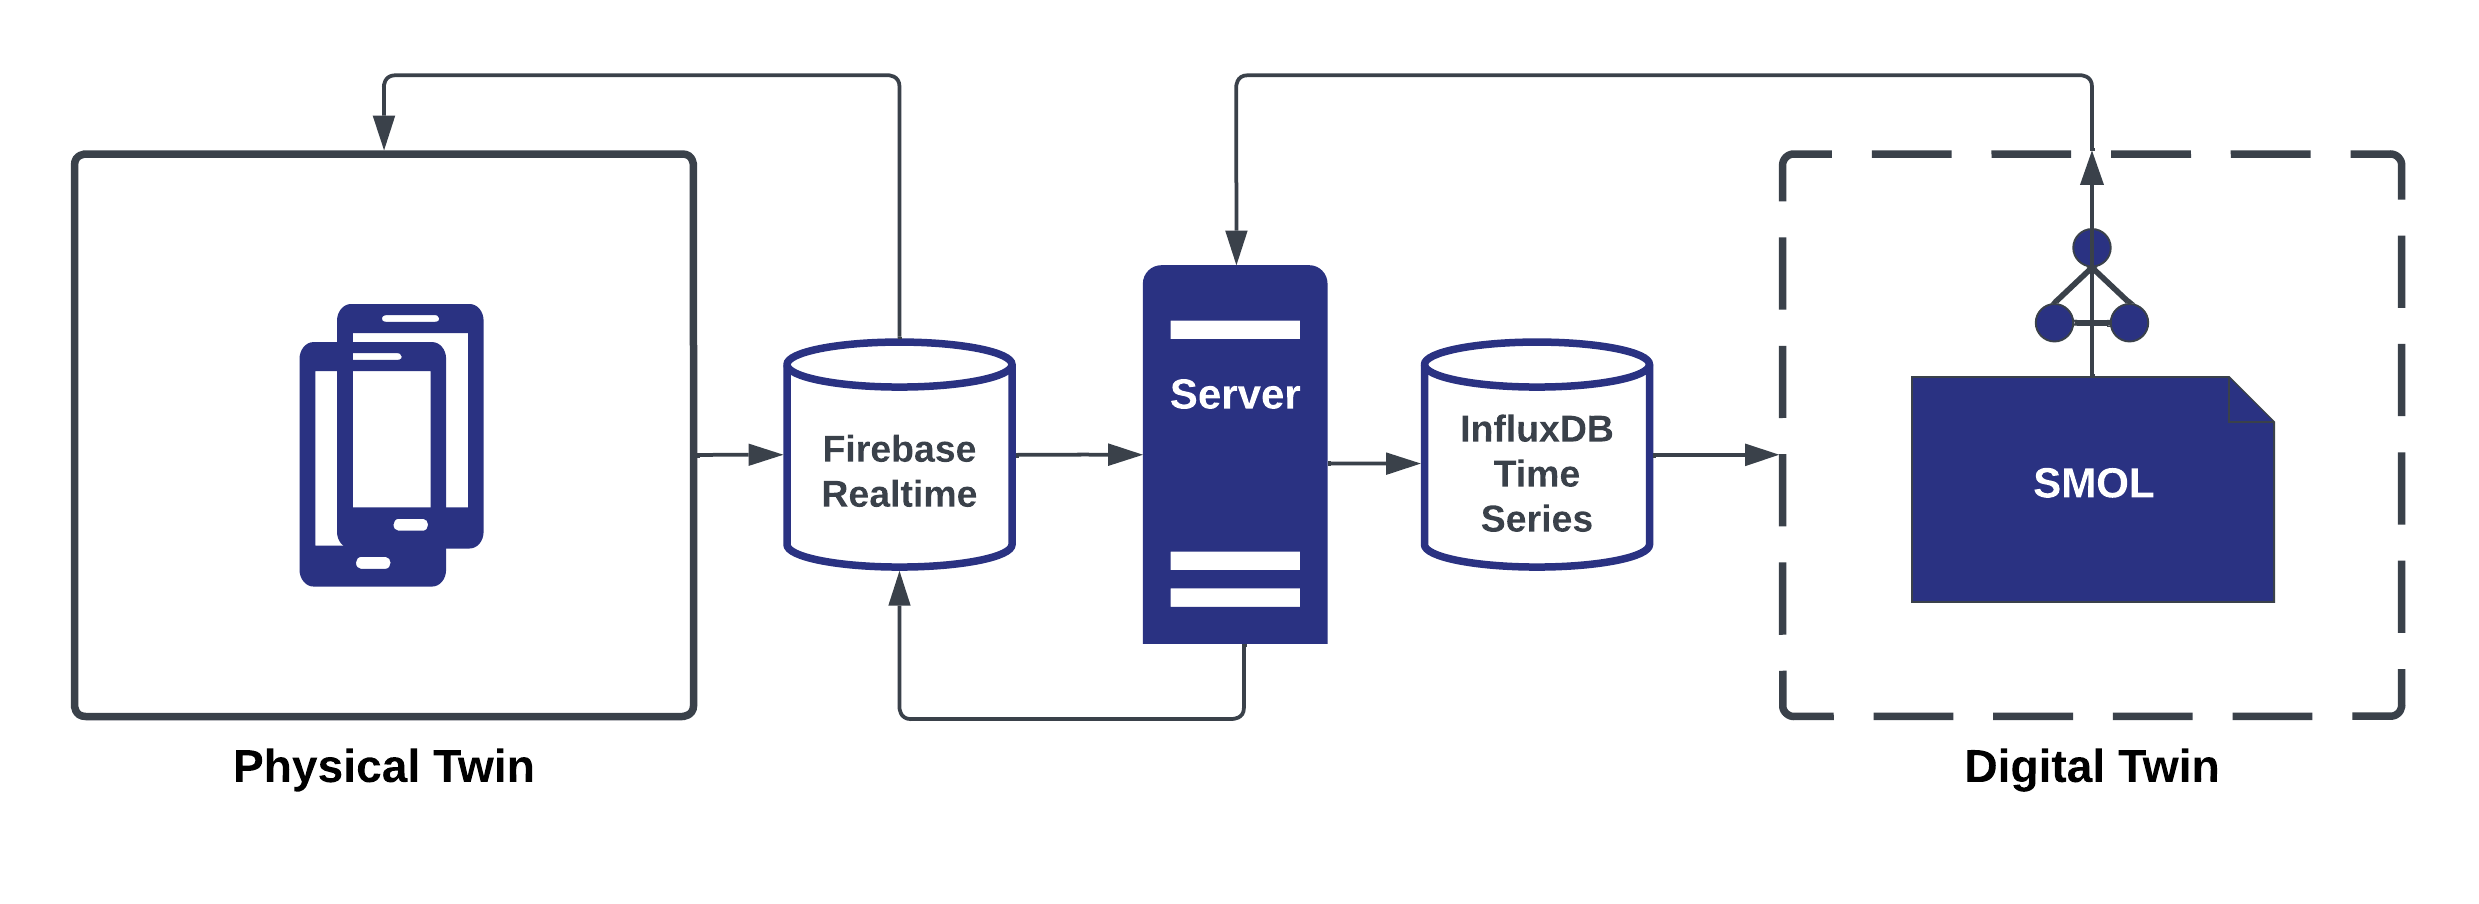
\includegraphics[scale=0.12]{graphics/thesis_overview.png}
    \caption{Possible overview of architectural components in this thesis.}
    \label{fig:components}
\end{figure}


\subsection{Thesis scope and outline}
The scope of this thesis is to handle an unlimited number of mobile assets in a semantic digital twin based on a dynamic asset model. Figure \ref{fig:components} shows the possible overview of architectural components and the bi-directional data flow between the PT and DT. The digital twin should be developed in Semantic Micro Object Language (SMOL)\footnote{\url{https://smolang.org/}} by using its interpreter \footnote{\url{https://github.com/smolang/SemanticObjects}}.
As noted by \citeauthor{pauwels_live_2023} many physical objects, such as furniture and doors, can be movable entities in a building apart from the robots. We limit ourselves to physical devices in 2D space. Doors will have one state (open). The areas are predefined squares with latitude and longitude ranges assuming the coordinates align. An area's two border corners are expressed as follows:
\begin{enumerate}
    \item $(x_1, y_1)$
    \item $(x_2, y_2)$
\end{enumerate}
Meaning, if we want to check if a smartphone's physical location (point) $(x, y)$ is inside such an area, we can check if the following is true:\newline\newline$(x >= x_1\:AND\: x <= x_2)\:OR\:(x >= x_2\:AND\:x <= x_1)$\newline$AND$\newline$(y >= y_1\:AND\:y <= y_2)\:OR\:(y >= y_2\:AND\:y <= y_1)$\include\newline We also include both directions so maintainers can freely choose border corners for an area. Square areas are easier to compute and scale into larger areas, and we are not focusing on other shapes such as polygons.\newline
Figure \ref{fig:simple_building} shows a simple building with two rooms connected by a wall with a door (open) in it.

\begin{figure}[!h]
    \centering
    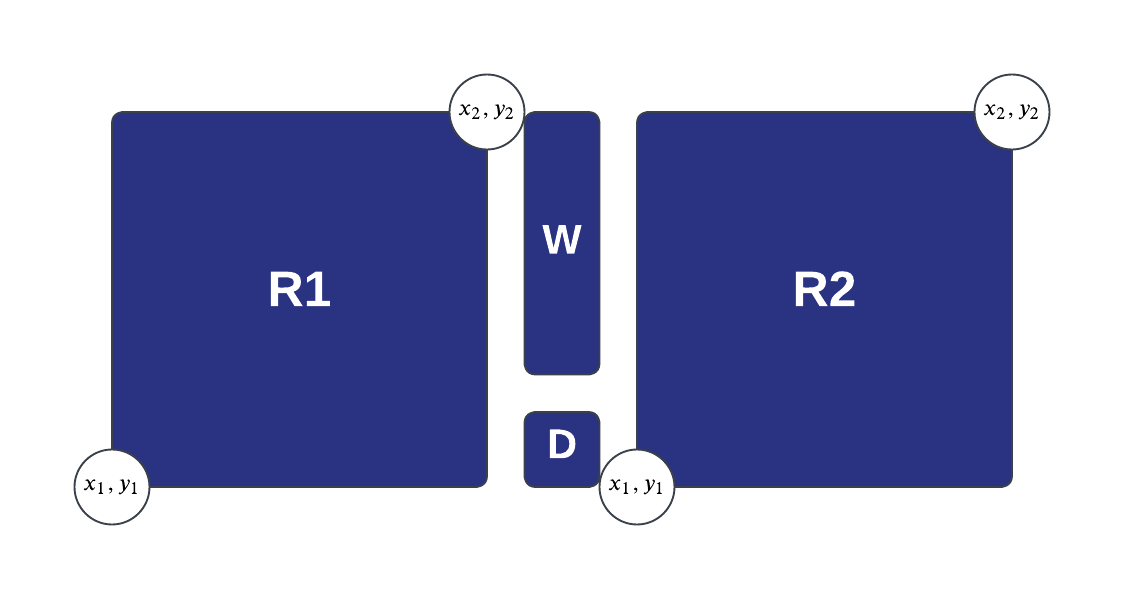
\includegraphics[scale=0.3]{graphics/simple_building.png}
    \caption{A simple building consisting of two rooms (R1 and R2) connected by a wall (W) with a door (D) in it.}
    \label{fig:simple_building}
\end{figure}


The remainder of this thesis is organized as follows:
\begin{itemize}
    \item \hyperref[sec:Background]{Background} describes the background of this thesis.
    \item \hyperref[sec:Analysis]{Analysis and design} investigates the problem statement and research questions. We also look at what a dynamic asset model entails, as well as the separation of static and dynamic data.
    \item \hyperref[sec:Implementation]{Implementation} looks into the implementation of the proposed solution and how the different architectural components outlined in Figure \ref{fig:components} interact. More specifically, how do we close the loop by sending informed decisions back to the PT. 
    \item \hyperref[sec:Evaluation]{Evaluation} evaluates the proposed solution according to the requirements that were set earlier.
    \item \hyperref[sec:Discussion]{Discussion} discusses the discoveries of this thesis and compares them to other existing results and theories, as well as explores the originality of the discoveries.
    \item \hyperref[sec:Conclusion]{Conclusion and further work} concludes this thesis. Mainly we look at the improvements that can be made to the proposed solution and the road ahead.  
\end{itemize}



\newpage
\section{Background}\label{sec:Background}
Short chapter intro about semantic web..

\subsection{Semantic Digital Twins}
\subsection{Apache Jena}
\subsection{OwlApi}
\subsection{Protégé}
\subsection{SparQL}
\subsection{Flutter}
\subsection{Google Maps SDK}
\subsection{SMOL}
\subsection{Databases}
\subsubsection{InfluxDB}
\subsubsection{Firebase realtime database}


\newpage
\section{Analysis and design}\label{sec:Analysis}
\subsection{Uncertainty quantification}
\subsection{Dynamic asset model}
\subsection{Data separation}
\subsubsection{Separate dynamic from static (from Rudi)}
Should this be in analysis and design?
\subsubsection{Separate static analysis from dynamic snapshots}
Separate static analysis of what is a critical area from dynamic snapshot of smartphones and critical area positions at a certain time, so dynamic is not affected (From Einar) (Should this be in analysis and design?)



\newpage
\section{Implementation}\label{sec:Implementation}

TODO: refer back to thesis scope
\begin{lstlisting}
Boolean hasPosition(Double lat, Double long)
    Boolean inAnyLatitudeRange = ((lat >= this.latitude1) & (lat <= this.latitude2)) | ((lat >= this.latitude2) & (lat <= this.latitude1));
    Boolean inAnyLongitudeRange = ((long >= this.longitude1 & long <= this.longitude2)) | ((long >= this.longitude2) & (long <= this.longitude1));

    if (inAnyLatitudeRange & inAnyLongitudeRange) then
        return True;
    end
    return False;
end
\end{lstlisting}


\subsection{Semantic Digital Twin}
\subsubsection{SMOL}
\subsubsection{Semantic Micro Object Language}
\subsubsection{Ontology}
\subsubsection{Querying}
\subsubsection{Digital Shadow}
\subsection{Client}
\subsubsection{Dart}
\subsubsection{Google Maps}
\subsection{Privacy}
\subsubsection{Position recording toggle}
\subsubsection{Permissions}
\subsection{Server}
\subsubsection{Java}
\subsection{Closing the loop (bidirectional communication between PT and DT)}
\subsection{Diagrams}



\newpage
\section{Evaluation}\label{sec:Evaluation}
\subsection{Test runs}
\subsubsection{Server automatically reloads asset model}
\subsubsection{Operator manually updates asset model}
\subsection{Plotting with Mermaid}
\subsection{User evaluation}
\subsubsection{Users}
\subsubsection{Test with many physical devices}
\subsubsection{Results}




\newpage
\section{Discussion}\label{sec:Discussion}




\newpage
\section{Conclusion and further work}\label{sec:Conclusion}
\subsection{Summary}
\subsection{Contributions}
\subsection{Further work}
\subsubsection{Writing to Influx directly from SMOL not possible and 'dump' limitation}
\subsubsection{Accuracy of position}
\subsubsection{Altitude}
\subsubsection{Point-in-polygon and Mercator projection}
\subsubsection{Anomaly detection}



\newpage
\printbibliography


\end{document}


